\def\pathToMain{../../buch/}
\documentclass{uebungsblatt}
\usepackage[utf8]{inputenc}
\usepackage[T1]{fontenc}
\usepackage[ngerman]{babel}

\usepackage{mathdef}
\usepackage{tikzdef}
\usepackage{multicol}

\sheet{Vorbereitungsblatt 15.1}
\title{Einführung: Lineare Gleichungen}
\topic{\getchaptername{lineare_gleichungen}}
\chapternum{\getchapternum{lineare_gleichungen}}

\begin{document}
\maketitle
\begin{contents}
    Unbekannte, Gleichungen
\end{contents}

\video{Variablen als Unbekannte}{4}{Kapitel \ref{ext:sec:abbildungen_intuition} (ab Seite \pageref{ext:sec:abbildungen_intuition})}{https://www.google.de}

\begin{definition}
    \parpic[r]{
        \tikz{
            \node at (0,0) {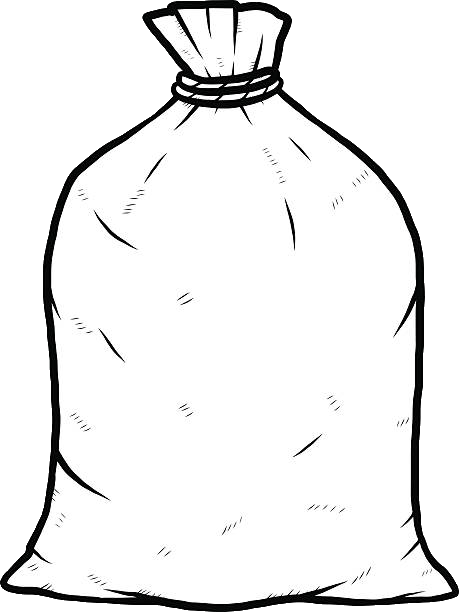
\includegraphics[height=2.8cm]{images/set_diagram.png}};
            \node[orange] at (0,0.4) {\scriptsize 4};
            \node[orange] at (0.3,-0.8) {\scriptsize 9};
            \node[orange] at (-0.3,-0.9) {\scriptsize 8};
            \node[orange] at (-0.2,-0.1) {\scriptsize 13};
            \draw[<-] (0.35,0.95) to[bend right] (0.8,1.4) node[above] {\scriptsize Menge};
        }
    }

    Eine \textbf{Menge} $M$ ist eine Zusammenfassung von unterscheidbaren Objekten, die die \textbf{Elemente} der Menge genannt werden. Ein Objekt $x$ heißt in der Menge $M$ enthalten, wenn es zu den Elementen der Menge $M$ gehört. In diesem Fall schreiben wir $x\in M$, ansonsten $x\notin M$.

    Zwei Mengen sind gleich, wenn sie die gleichen Elemente enthalten. Eine Menge, die keine Elemente enthält, wird als \textbf{leere Menge} bezeichnet und mit dem Symbol $\emptyset$ notiert.
\end{definition}
\end{document}
